\chapter{Background}
\lhead{\emph{Background}}

Given the increasing prevalence of information systems and information science in general, data volumes continue to grow exponentially\cite{Devakunchari}. Much of the data consumed by information processing systems is now generated by automated processes such as networks of sensors, financial transaction management systems and telephony networks. These system produce \textit{data streams}, unbounded datasets which update continuously over time. A data stream is defined by \citeauthor{data_stream_processing} as \textit{"an ordered sequence of instances that can be read only once or a small number of times using limited computing and storage capabilities"}\cite{data_stream_processing}.

\textit{Stream processing} has emerged in recent years as an approach to the design of software systems responsible for the real-time processing of such data streams\cite{Andrade:2014:FSP:2823980}. In contrast to batch-oriented Data Warehousing systems, which typically persist volumes of data for processing at some point in the future, stream processing systems continuously consume inputs, producing corresponding and continuous streams of outputs. 

Several domains are intrinsically suited to the real-time processing of data streams; in particular, those domains in which timely response to insights yielded by real-time processing presents business value. The \textit{sense-and-respond pattern}, a concept borrowed from control theory, has been used to describe the process of deriving continuous streams of business intelligence by means of real-time stream processing\cite{Nguyen:2005:SRS:1097002.1097015}. Domains which frequently leverage the sense-and-respond pattern include financial fraud detection, threat detection, and Internet of Things (IOT) data analytics.

For financial fraud detection, minimisation of the time delta between transaction data consumption and the production of corresponding analytics or alerts is critical. \citeauthor{Nguyen:2005:SRS:1097002.1097015} have proposed an approach to financial fraud detected entitled Sense and Response Service Architecture (SARESA), underpinned by an event-driven architecture which continuously consumes data streams from a business environment\cite{Nguyen:2005:SRS:1097002.1097015}. The authors contrast their proposed design with the typical Data Warehouse architecture, which stages data streams to a persistent database in order to perform aggregation and reporting at a later time; SARESA in comparison continuously ingests, transforms, and processes events in real-time. At the implementation level, SARESA comprises a pool of independent services communicating over a shared message bus. The use of a message bus provides for decoupling of services and lends a high degree of adaptiveness to the system;  \citeauthor{Nguyen:2005:SRS:1097002.1097015} assert that "\textit{..the processing steps of a Sense and Respond loop can be flexibly changed and updated}".

An event-driven, real-time stream processing pipeline will typically comprise a set of distributed microservices, a common architectural choice in the design and implementation of data pipelines\cite{pipeline_microservices}. \citeauthor{Cerny_microservices} consider microservices in the context of the Unix design philosophy, identifying the following three qualities of the architecture\cite{Cerny_microservices}:

\begin{enumerate}
	\item A microservice performs a dedicated task, and performs it well.
	\item A microservice interoperates with other microservices.
	\item A microservice communicates with other microservices over a universal interface.
\end{enumerate}

Two factors suggesting the suitability of microservices for pipeline implementation are potential for horizontal scalability and the inherently decoupled nature of the microservices themselves\cite{Hasselbring}.  Scalability is necessary in order to minimise pipeline processing delays when dealing with high volume data streams; furthermore the ability to scale down a pipeline is desirable during periods of minimal stream volume, in order to minimise resource consumption.

Service decoupling is achieved through use of a distributed messaging system,  as proposed by  \citeauthor{Nguyen:2005:SRS:1097002.1097015}. While pipeline microservices interact with each other, they do not do so directly and are generally unaware of each other. Rather, interaction is performed using a messaging system. As such, message data defines the contract between pipeline microservices. Distributed messaging systems typically leverage a publish-subscribe model, where message producers write to a \textit{topic}, while message consumers \textit{subscribe} to a topic. Producers are unaware of the set of message consumers, and conversely, the consumer of a message or event is unaware of the producer of same. This service decoupling lends a great deal of flexibility to pipeline design, with considerable scope for pipeline evolution over time, as will be explored later in this chapter. Popular contemporary messaging systems include Apache Kafka\cite{ApacheKafka}, ActiveMQ\cite{ActiveMQ} and RabbitMQ\cite{RabbitMQ}. 

Threat detection systems perform a broadly similar function to fraud detection systems, processing data streams continuously in order to generate real-time threat alarms and response action triggers. 
Figure \ref{threat_detection_pipeline} describes a simplified threat detection pipeline.

\vspace{5mm}

\begin{figure}[H]
	\centering  
	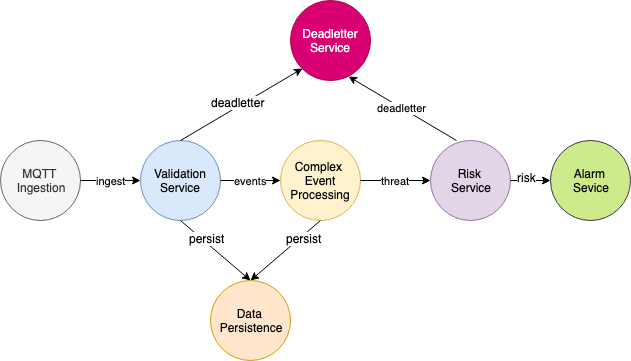
\includegraphics[scale=0.6]{figures/background/threat_detection_pipeline.png}
	\caption{Simple threat detection pipeline.}
	\label{threat_detection_pipeline}
\end{figure}

\begin{itemize}
	\item MQTT events from IoT devices are ingested at the \texttt{MQTT Ingestion Service}, transformed to an internal event/message representation, and forwarded to an \texttt{ingest} event channel.
	\item The \texttt{Validation Service} performs validation operations on events received. Some events may contain declarations of newly discovered IoT device metadata; such events will be forwarded to a \texttt{persist} event channel. Some events may represent for instance alarms generated by external IoT device such a window breakage alarm; these events are forwarded to the  \texttt{events} message channel. Uninteresting messages are discarded by forwarding them to a \texttt{Deadletter} channel.
	\item The \texttt{Complex Event Processing Service} consumes messages from \texttt{events} channel and performs processing based on for instance a rule engine definition or set of Machine Learning (ML) algorithms. Those events determined to to represent a threat are transformed to \texttt{Threat} events and forwarded to the \texttt{threat} channel. 
	\item The \texttt{Risk Service} processes incoming \texttt{Threat} events and depending on various criteria, may forward a new event on the \texttt{risk} channel.
	\item The \texttt{risk} event channel has a single consumer, the \texttt{Alarm Service}, responsible for real-time reporting of events to organisational security personnel in the event that a risk notification meeting certain criteria (for example, a numeric risk score in excess of a defined threshold) is encountered.
	
\end{itemize} 


A key aspect of this architecture is that no explicit contract is defined between microservices. As events flow through the pipeline, no event publisher is aware of consuming services. This trivialises the process of adding additional flows to a pipeline, for example:

\begin{itemize}
	\item New event types may be handled by adding an additional microservice which listeners to the \texttt{ingest} message channel.
	\item \texttt{Risk} event duplication may be eliminated by introduction of a \texttt{Correlation} microservice, which listens to the \texttt{threat} message channel, removing duplicates before fowarding to a new \texttt{threat-dedup} channel.
\end{itemize}

In order to implement these changes, the only code or configuration changes necessary for \textit{existing} microservices may be as minimal as reconfiguring the \texttt{Risk Service} to subscribe to \texttt{threat-dedup} rather than \texttt{threat} events. While this flexibility confers several benefits in terms of architectural flexibility and potential for pipeline evolution, it creates challenges with regards to determination of pipeline topology at a given moment in time, in particular during the development phase of product life-cycle.


\section{Literature Review}

While the author has reviewed several publications pertaining to discovery of Microservice Architecture based application structures, there appears to be a paucity of literature surrounding real-time topography discovery and message activity summarisation for message-driven data pipelines. What literature is extant largely explores the discovery and monitoring of microservice-based applications, a more general area.

 \citeauthor{8359145} have explored a method for automatic derivation of MSA-based application structures in \cite{8359145}. The approach described involves a combination of static service and API analysis coupled with data collection during application runtime. The system described in \cite{8359145} resembles the architecture proposed in this Chapter 3 of this thesis in so far as it comprises several cooperating modules. An \textit{Aggregation Service} aggregates data collected during runtime, while a \textit{Management Service} stores information about the described application architecture. A \textit{Data Collection Library} is used to instrument microservices in order to automatically generate runtime data. \citeauthor{8359145} suggest that the primary use cases for their proposed system lie in the domains of creating architecture documentation, analysing architectural evolution, and supporting architectural change.

The system described is compatible with Spring microservices exclusively, and metrics generated pertain to REST communication only. No support is provided for message-based MSA applications; ``\textit{Indirect communication using message queues or some other kind of message-based middleware is currently not supported by our approach}'' \cite{8359145}. Generated metrics include workload response time, service response time, and error rates.  \citeauthor{8359145} furthermore demonstrate several dashboard widgets which present historical application metrics including failure rates over all services, error response code distribution, and service-to-host allocation information.  As REST communication is the only mode of inter-service communication monitored by this solution, it  is not applicable as regards monitoring of message-drive pipelines.

\citeauthor{8548311} describe a non-invasive approach to microservice monitoring in \cite{8548311}; no microservice source code modification or instrumentation is necessary. Leveraging the observation that service discovery is a common pattern in MSA applications, the authors propose instrumenting popular load balancing and service discovery service implementations developed by Netflix. In doing so, an instrumented gateway is used to gather metrics based on as response times, request source and destination addresses, invoked REST API functions and the like. Furthermore, failure detection is performed by inspection of the container runtime environment which hosts the analysed application services. Much like the work described in \cite{8359145}, this monitoring solution is not usable with applications based on asynchronous messaging, a common architecture for data-pipeline applications. \citeauthor{8548311} describe a front-end module used to render static application dependency graphs and various metrics including response time by microservice and latency between services.

\citeauthor{8530769} explore an alternative approach to non-invasive microservice communication monitoring is explored in \cite{8530769}. \textit{MetroFunnel} sniffs network traffic in order to analyse inter-service REST request-response messages. A trace log containing various metrics including invocation processing times, error response codes and timeout statistics is generated by the tooling. No dashboard functionality, real-time or otherwise, is presented. This monitoring approach may suffer a serious shortcoming in that it presupposes third-party access to network traffic between microservices, which is often not practical. Further, MetroFunnel is limited to analysis of REST HTTP traffic only, a shortcoming shared with the proposals presented in \cite{8359145} and \cite{8548311}. This approach cannot currently be applied to topology discovery or message activity monitoring in message-driven data pipelines.

\textit{Pink}, a system for synthetic runtime monitoring of MSA applications based on scripts generated from annotated UML diagrams is described in \cite{8377902}.  \citeauthor{8377902} propose that users of Pink model a given application using UML component and sequence diagrams, annotating those models with constraints expressed in Object Constraint Language (OCL). These models are then used to generate a series of monitoring scripts which synthetically enumerate describe both possible interactions between microservices, and possible microservice states. Issues with state-space explosion aside, this approach has no applicability to runtime pipeline monitoring, as it concerned with a synthesised enumeration of possible application states only. 

\section{Current State of The Art}

In the author's experience, the cluster of console windows depicted in Figure \ref{console_monitoring} is a common sight in development labs. Each window is listening to an individual message channel or topic in a deployed pipeline application. A developer or test engineer may be attempting to pinpoint the point of failure in a pipeline, or perhaps establish whether there is activity on any part of a pipeline. This approach to pipeline monitoring is thoroughly unwieldy.

\begin{figure}[H]
	\centering  
	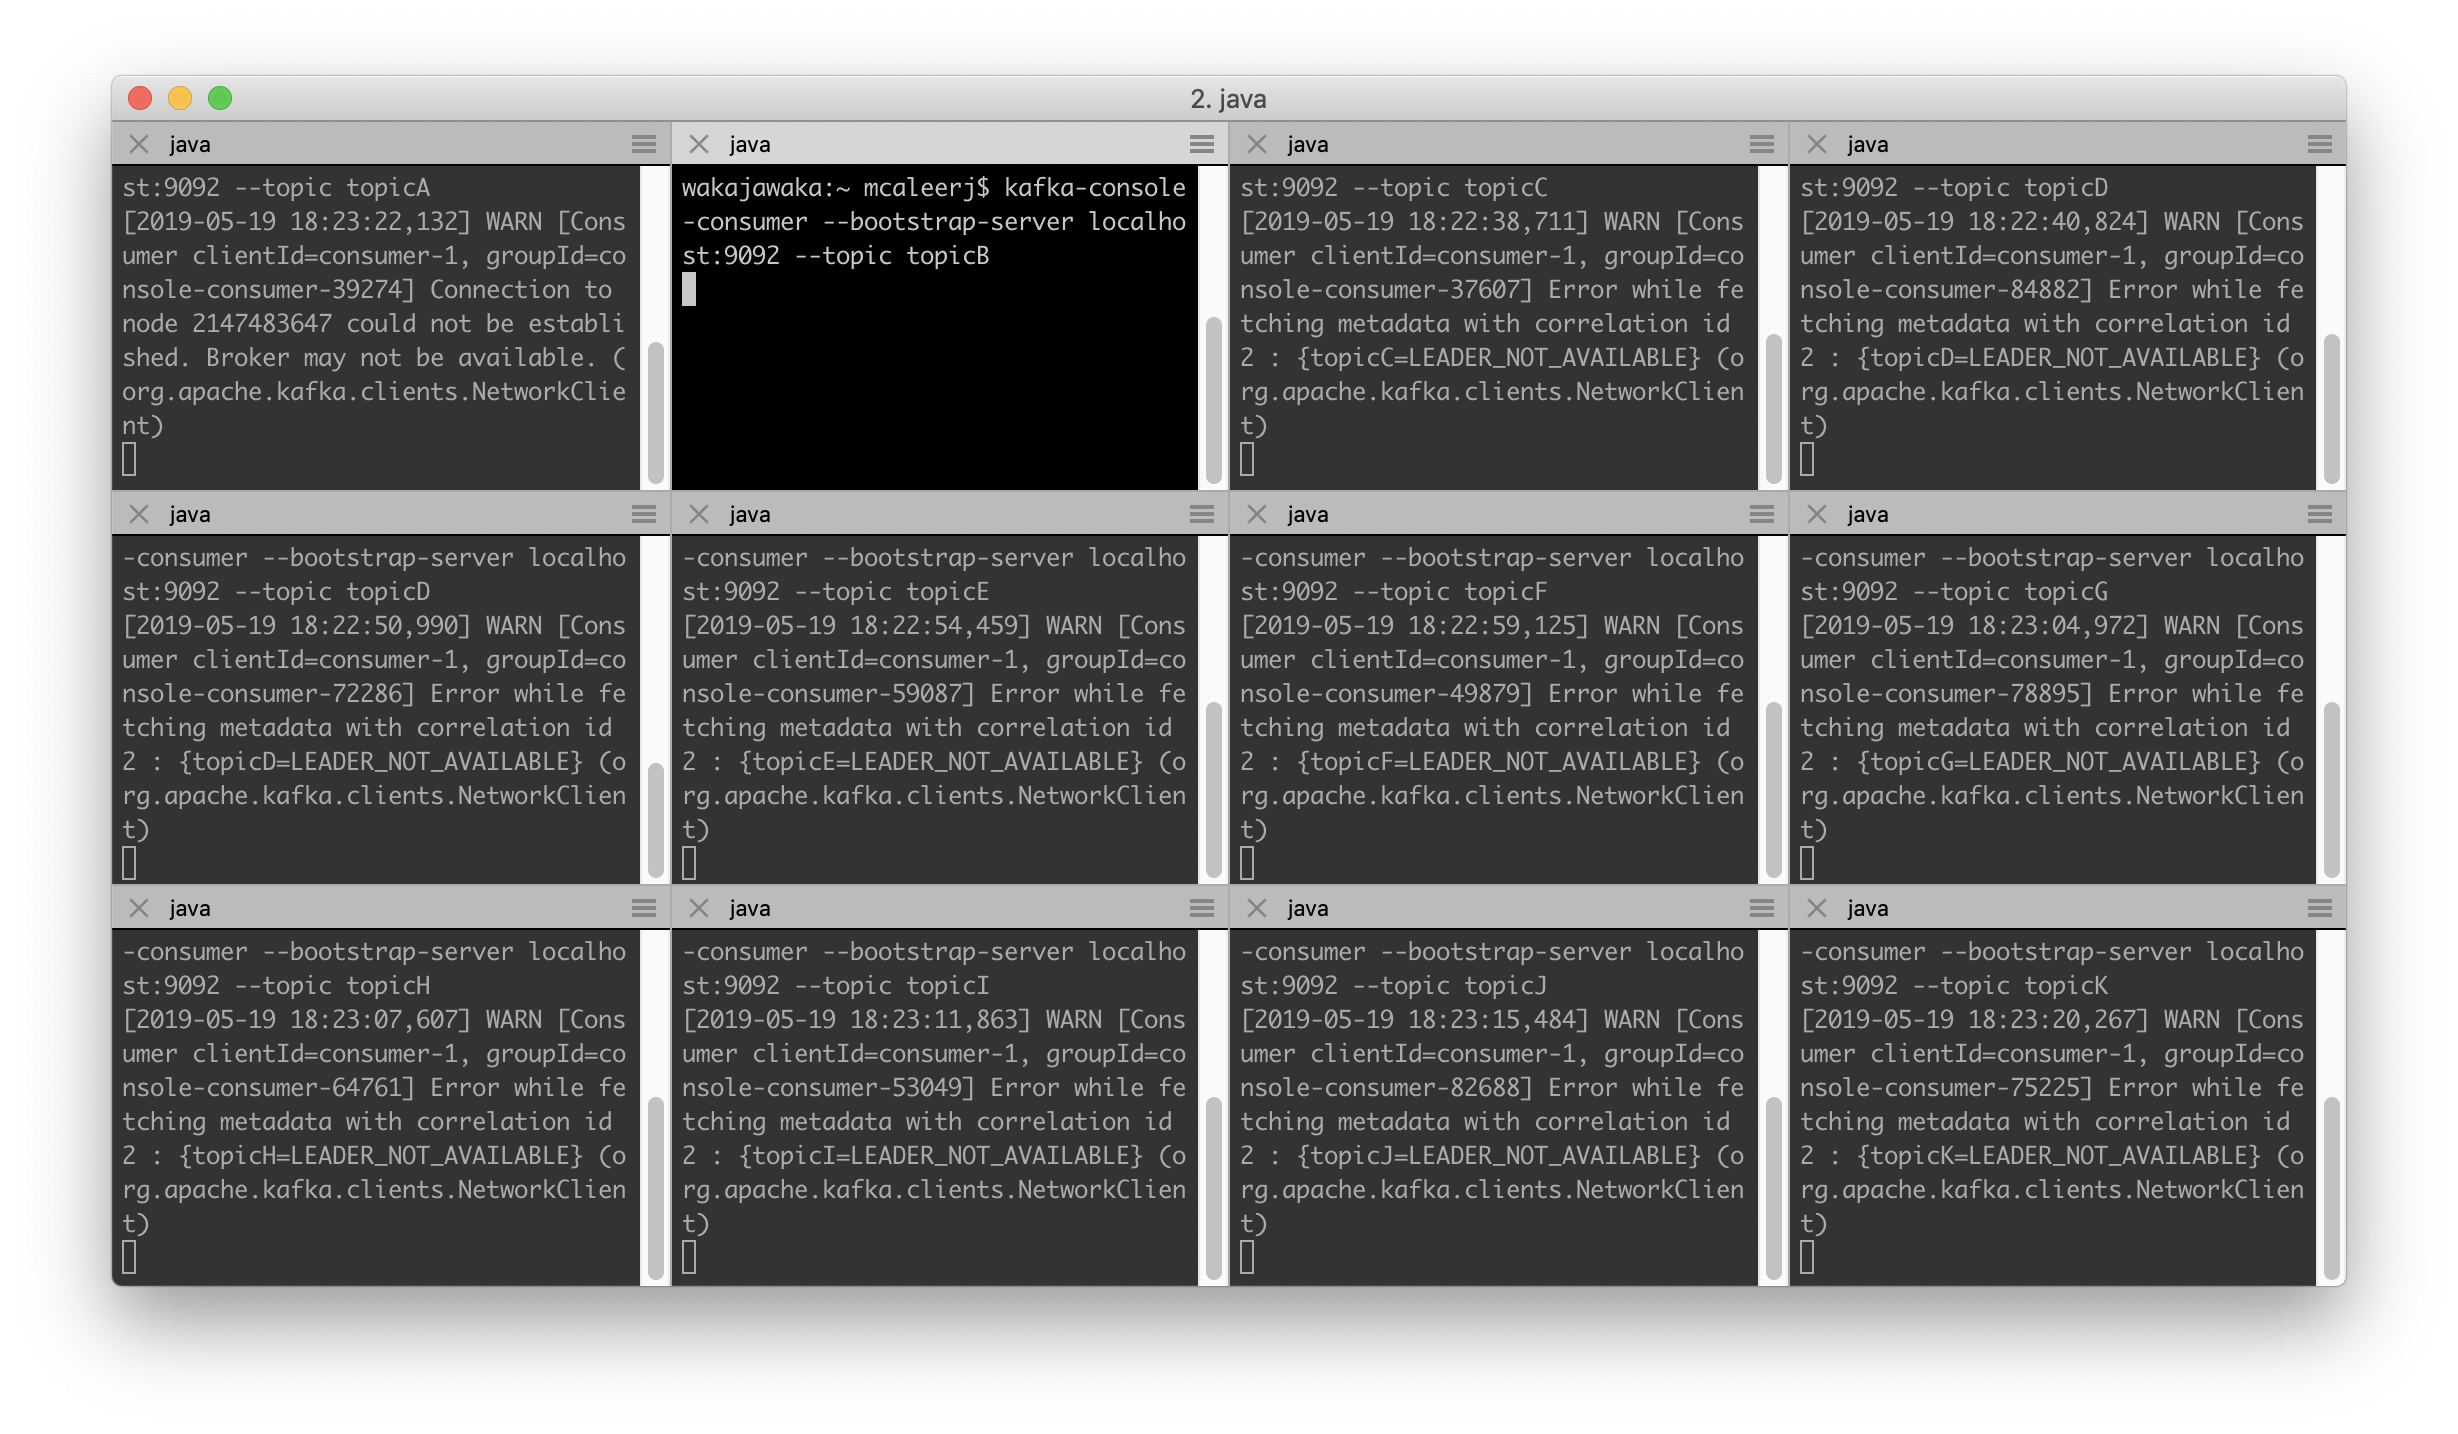
\includegraphics[scale=0.3]{figures/background/monitoring.png}
	\caption{Numerous consoles listening on Kafka topics.}
	\label{console_monitoring}
\end{figure}

With the growth of big data and related disciplines, data pipelines have become an increasingly popular design paradigm; consequently various real-time pipeline monitoring solutions have become available in recent years. Likewise major cloud service vendors now offer a variety of message-driven data pipeline frameworks and accompanying monitoring solutions. In this section, several open-source and proprietary monitoring products will be discussed and compared with the approach and solution proposed by this thesis. 

\subsection{Amazon CloudWatch}
Amazon Managed Streaming for Kafka (Amazon MSK) - is Amazon's managed, Kafka-based service for processing of continuous data streams\cite{AmazonMS34:online}. The offering is currently in its infancy and at time of writing, in public preview. Amazon's corresponding monitoring solution is \textit{Amazon CloudWatch}, which enables collection of metrics such as messages per unit time sent by message producers, the number of network packets transmitted per unit time, log sizes, CPU usage, and the like. As such, Amazon CloudWatch provides no topology discovery functionality whatsoever, and while it collates various metrics at the network and message broker level, does not provide dashboards which convey at a high level, messaging activity across a pipeline. The CloudWatch dashboard interface depicted in Figure \ref{cloudwatch_ui} demonstrates the metrics-focused nature of the solution.

\vspace{5mm}

\begin{figure}[H]
	\centering  
	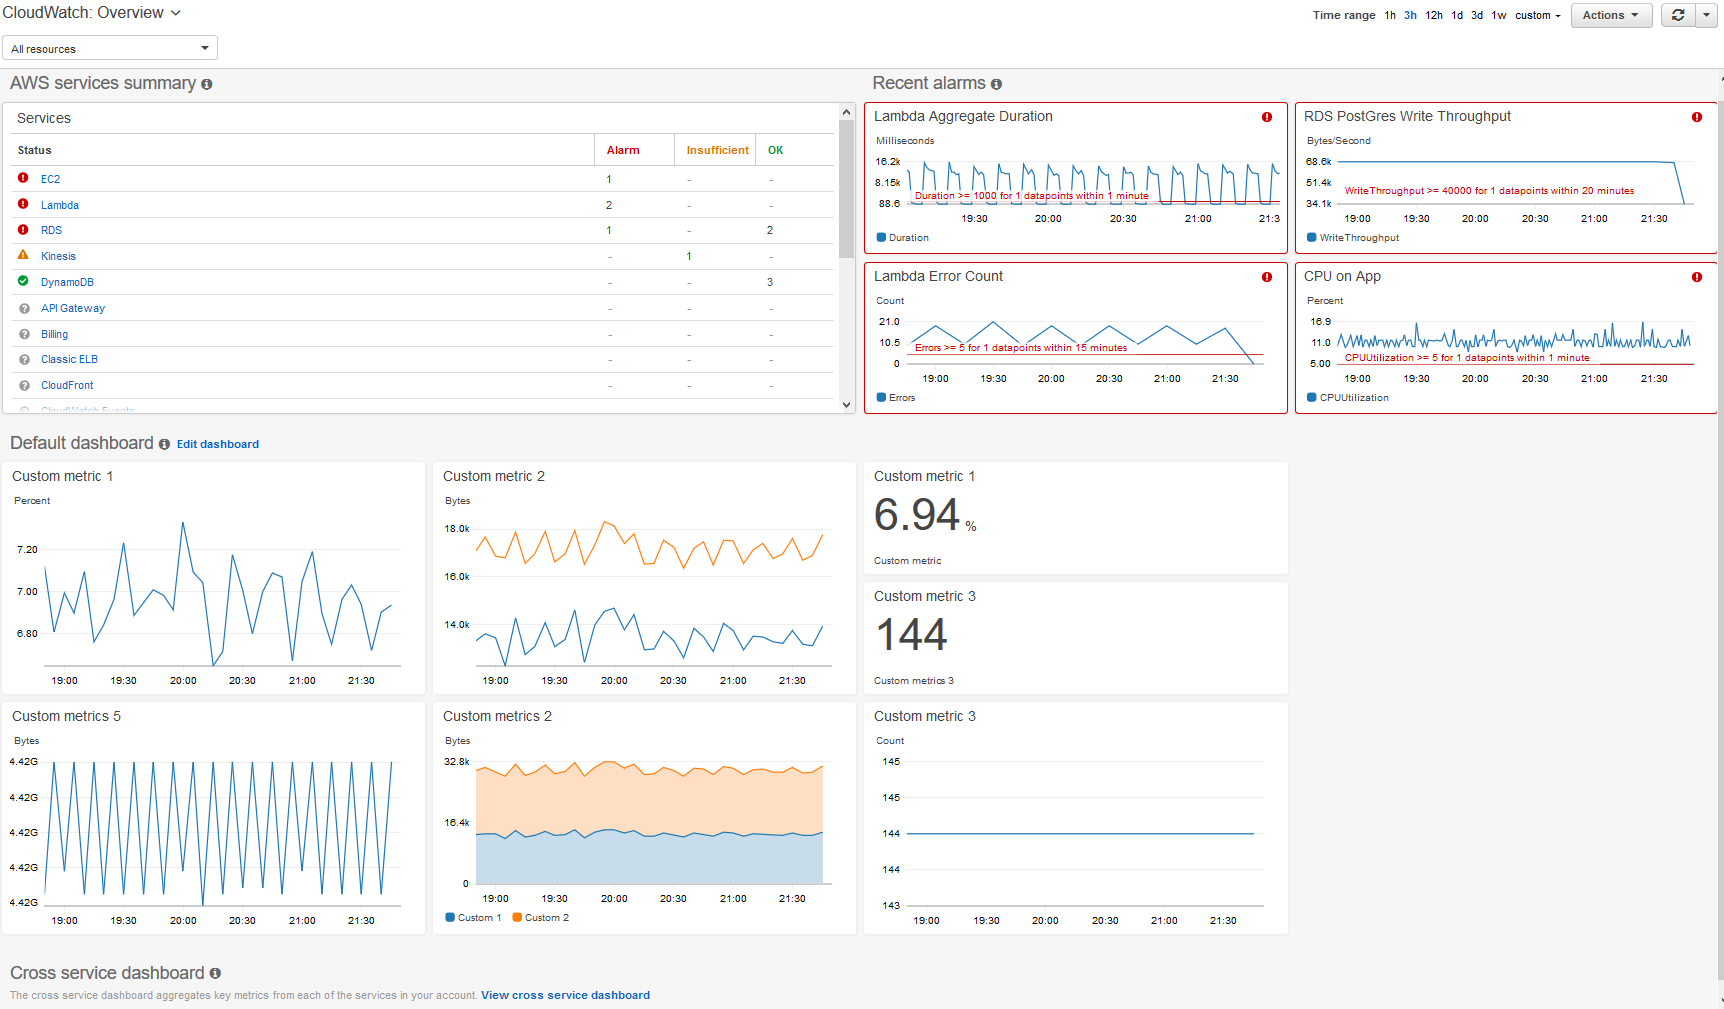
\includegraphics[scale=0.4]{figures/background/cloudwatch.png}
	\caption{Amazon CloudWatch monitoring dashboard.}
	\label{cloudwatch_ui}
\end{figure}

\subsection{Azure Dashboards}
Microsoft's current offerings around implementation of data pipelines are \textit{HDInsight},  \textit{Stream Analytics}, and  \textit{Data Factory}, which variously support implementation of Kafka-based applications, data transformation pipelines, and event processing engines in general. Microsoft enable the creation of monitoring dashboards within the Azure portal; such dashboards can be configured to leverage metrics around pipeline availability and overall pipeline health. The metrics made available correspond to those exposed by Amazon's monitoring solution; CPU usage, network usage, message broker statistics and the like. This metric-centric monitoring solution, like Amazon's \textit{CloudWatch} service, has scarce potential to address the central use case of the solution proposed by this thesis, namely: \textit{As a developer, I want to understand the composition and activity state of my deployed pipeline applications at a glance}. 

Pipeline monitoring solutions offered by the larger cloud players such as Amazon and Microsoft clearly target an Enterprise IT Operations Management (ITOM) audience, concerned primarily with \textit{five nines} availability and application performance. A number of commercial and open-source monitoring solutions focused on topology discovery and pipeline activity monitoring have however emerged in recent years.

\subsection{Lightbend OpsClarity}
\textit{OpsClarity} is a commercial, closed-source software product positioned specifically for real-time data pipeline monitoring\cite{OpsClarity}. OpsClarity reports on a plethora of real-time metrics including pipeline throughput, latency, error rates and data loss.  This solution integrates with a number of popular frameworks including Apache Kafka, Apache Zookeeper, Apache Spark, MongoDB, and Docker. In addition to reporting various pipeline metrics, OpsClarity features automated topology discovery and real-time visualisation for various supported technologies - features which mirror the cornerstone goals of this research. While specific details of how activity monitoring topology discovery is performed are not made available by the product vendor, product documentation does state that discovery and monitoring functionality is implemented by a series of agents \cite{OpsClarity_agents}. Agent installation is required per monitored host. While the monitoring solution proposed in this thesis will likewise be agent and plug-in based, as proposed in Section \ref{exec_summary}, it will not by contrast require configuration or instrumentation of monitored host environments.

In further contrast with the monitoring software proposed by this research, the OpsClarity solution performs activity monitoring at a higher level of granularity. OpsClarity monitors traffic flow between high-level components such as Kafka clusters, Apache Spark engines, Memcache instances, and ElasticSearch instances. While the range of metrics generated by the software is comprehensive, it does not perform topology discovery for microservices communicating within a messaging cluster. This is a key distinction between OpsClarity's offering and the work proposed in this thesis; the prototype developed as part of this dissertation will monitor and reflect messaging activity and pipeline topology \textit{within} for instance a Kafka cluster. The OpsClarity solution regards a Kafka cluster as an atomic entity, communicating with other components of a distributed data pipeline, such a CEP engines, database systems and distributed caches. In continuing contrast, the OpsClarity solution does not provide real-time dashboard visualisation of message aggregation data between pipeline microservices. 

As such, the intended target audience of this offering is an ITOM audience; OpsClarity is not positioned to satisfy the use case stated in the introductory chapter of this thesis, i.e. \textit{As a developer, I want to understand the composition and activity state of my deployed pipeline applications at a glance}.

\subsection{Apache StreamSets}

\textit{StreamSets} is an open source, Apache-licensed framework used for the design, execution and real-time monitoring of data pipelines. Pipeline design an an integral aspect of StreamSets, which features an advanced drag-and-drop UI for pipeline topology design, as depicted in Figure \ref{streamsets_design_ui}. 

\vspace{5mm}

\begin{figure}[H]
	\centering  
	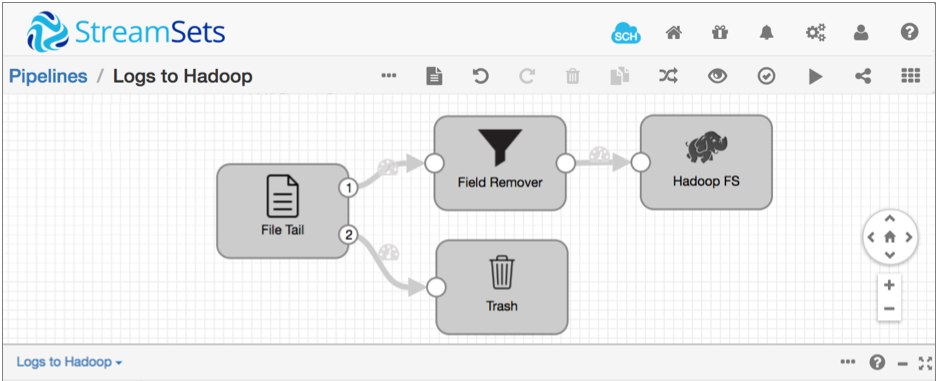
\includegraphics[scale=2.0]{figures/background/streamsets_design_ui.png}
	\caption{StreamSets pipeline topology designer.}
	\label{streamsets_design_ui}
\end{figure}

In contrast with the monitoring solution proposed in this thesis, StreamSets is an encompassing solution, targeting all phases of pipeline lifecycle from design to implementation and monitoring. StreamSets does not feature any form of topology discovery, as pipeline structure is input during the topology design phase of pipeline life-cycle. Moreover, in stark contrast to the proposed monitoring solution, StreamSets cannot be used to monitor a pipeline implemented \textit{without} use of the framework. 

The StreamSets monitoring user interface does not display metrics per message channel or topic, nor does it render channel or topic names; a directed graph representation denotes the sender and consumer of messages only. As such, the monitoring functionality may have limited use as a general-purpose environment monitoring dashboard when framed in the context of questions enumerated in Section \ref{intro_motivation}. The user interface is relatively dense and given the proliferation of controls presented in Figure \ref{streamsets_monitor_ui}, clearly intended for interactive use. Once again revisiting the key use case stated in the introductory chapter - \textit {As a developer, I want to understand the composition and activity state of my deployed pipeline applications at a glance} - StreamSets, while evidently a powerful and popular framework\cite{StreamSe68:online}, does not meet this requirement.

\vspace{5mm}
 
\begin{figure}[H]
	\centering  
	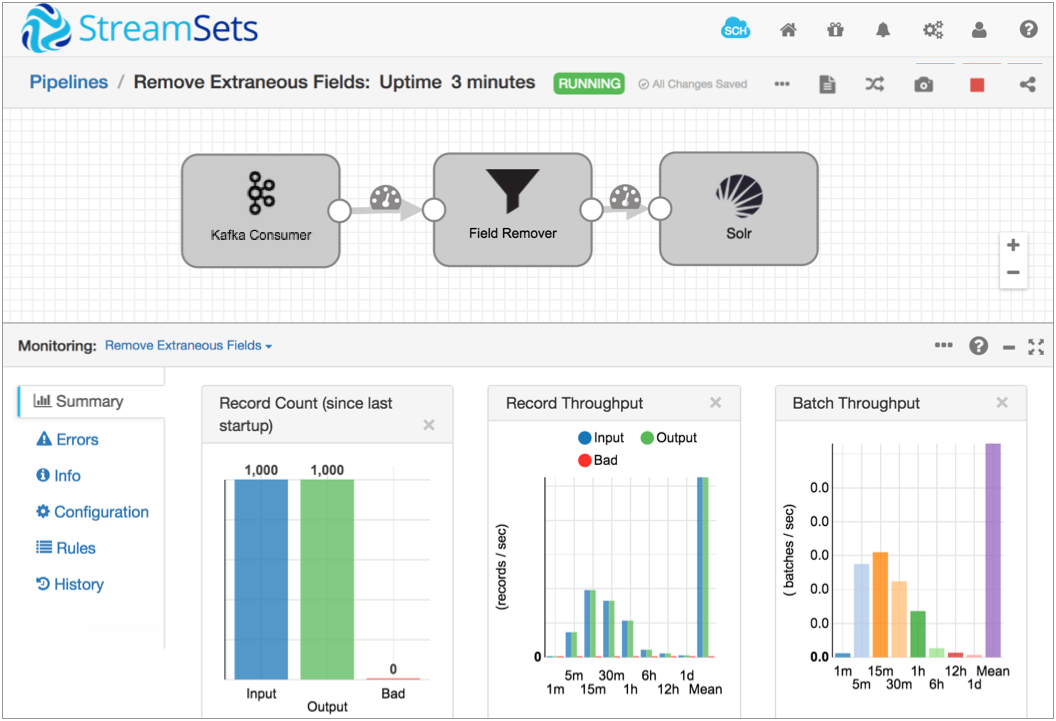
\includegraphics[scale=1.4]{figures/background/streamsets_monitor_ui.png}
	\caption{StreamSets real-time monitoring UI.}
	\label{streamsets_monitor_ui}
\end{figure}

\subsection{Kiali}

\textit{Kiali}, a GitHub-hosted open-source project (https://github.com/kiali/kiali), aims to provide answers to the question: What microservices are part of my Istio service mesh and how are they connected\cite{kiali_online}? Kiali delivers real-time interactive graphs of microservice interactions via interrogation of an \textit{Istio Service Mesh}. Istio documentation defines a service mesh as "\textit{... the network of microservices that make up such applications and the interactions between them}"\cite{Istio_mesh_online}. Istio essentially augments a set of microservices by directing all microservice inter-communication though per-service \textit{sidecars}, intelligent proxies responsible for traffic mediation. A separate Istio \textit{control plane} manages load balancing, routing rules, rate limiters, metric generation and security functionality\cite{Istio_mesh_online}.

Kiali performs pipeline topology discovery and activity monitoring via interrogation of the Istio control plane. Directed graphs are used to render mesh topologies as depicted in Figure \ref{kiali_monitor_ui}; the solution provides inter-service traffic visualisation by animating the edges connecting graph nodes. While this approach achieves the major goals outlined in this research - namely, real-time monitoring and rendition of both data pipeline topology and message activity - pipeline integration with Istio is a prerequisite, which may prohibit use in some environments. Furthermore, the Istio dependency inherently implies a transitive dependency to Kubernetes - prohibiting use of this monitoring solution in alternate environments. While comparatively limited in scope - Kiali enables monitoring of various inter-service communication media - the solution presented in this dissertation is technology-agnostic and considerably more lightweight.

\begin{figure}[H]
	\centering  
	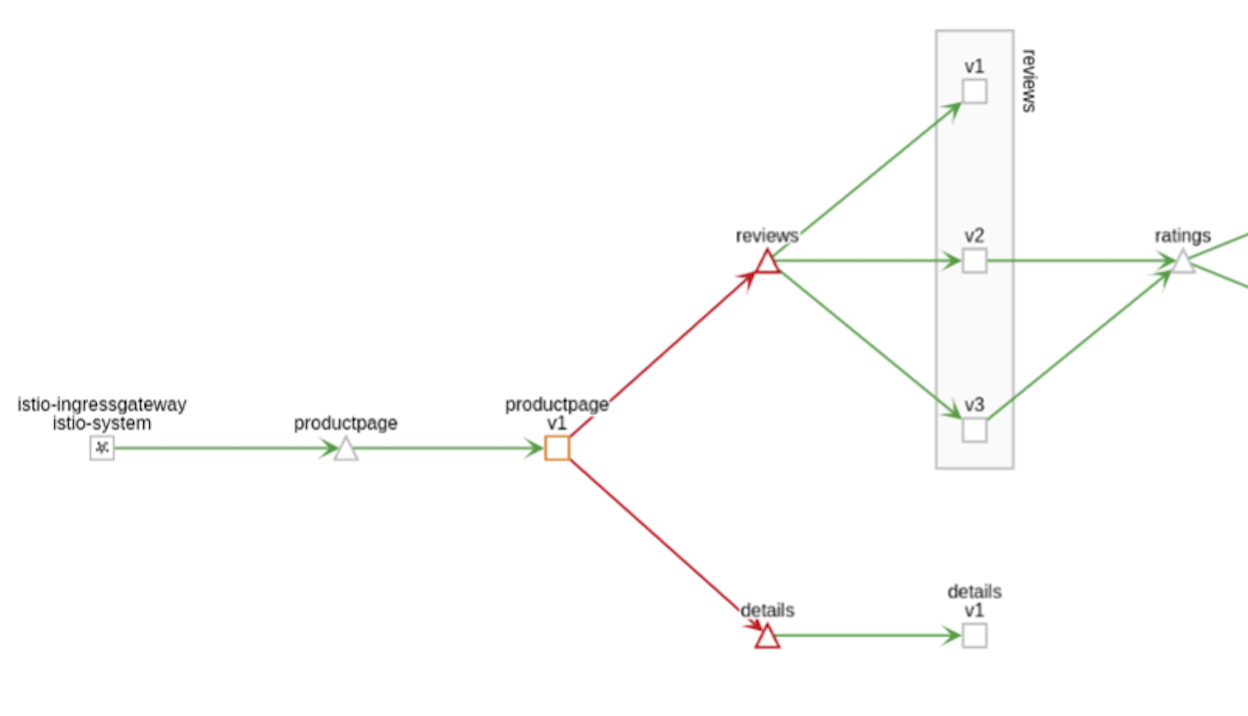
\includegraphics[scale=1.4]{figures/background/kiali.png}
	\caption{Kiali real-time monitoring UI.}
	\label{kiali_monitor_ui}
\end{figure}

In summary, of the real-time pipeline monitoring solutions discussed above, Kiali is alone in featuring both real-time topology discovery and per-message channel activity reporting. As such, of the existing software explored here, it is the only viable successor to the array of console windows depicted in Figure \ref{console_monitoring}.

To contrast Kiali against the solution described by this thesis, the proposed implementation will have relatively few dependencies; monitoring of a Kafka-based pipeline should for instance require details of the Kafka bootstrap server address only. Kiali meanwhile requires full Istio and Kubernetes integration for pipeline deployments. The solution proposed here will be further differentiated by its use of a simple, focused dashboard which clearly communicates information satisfying the basic use case started in the opening chapter. As that use case states, the use case actor in question is not in an ITOM role, but is more likely a software developer or tester. 
